\chapter{Exploratory Data Analysis (EDA)}

\section{Overview \& Visual Philosophy}
Exploratory Data Analysis (EDA) forms the foundational diagnostic phase of Data Mining. EDA identifies underlying empirical distributions, uncovers non-linear feature interactions, detects potential anomalies, and provides clinical domain context before machine learning model training.

\section{Target Variable Class Distribution}
Figure~\ref{fig:eda_target} illustrates the target variable class balance ($N=9,000$). Healthy controls ($0$) represent $69.7\%$ ($6,273$ patients) whereas heart disease cases ($1$) represent $30.3\%$ ($2,727$ patients).

\begin{figure}[H]
\centering
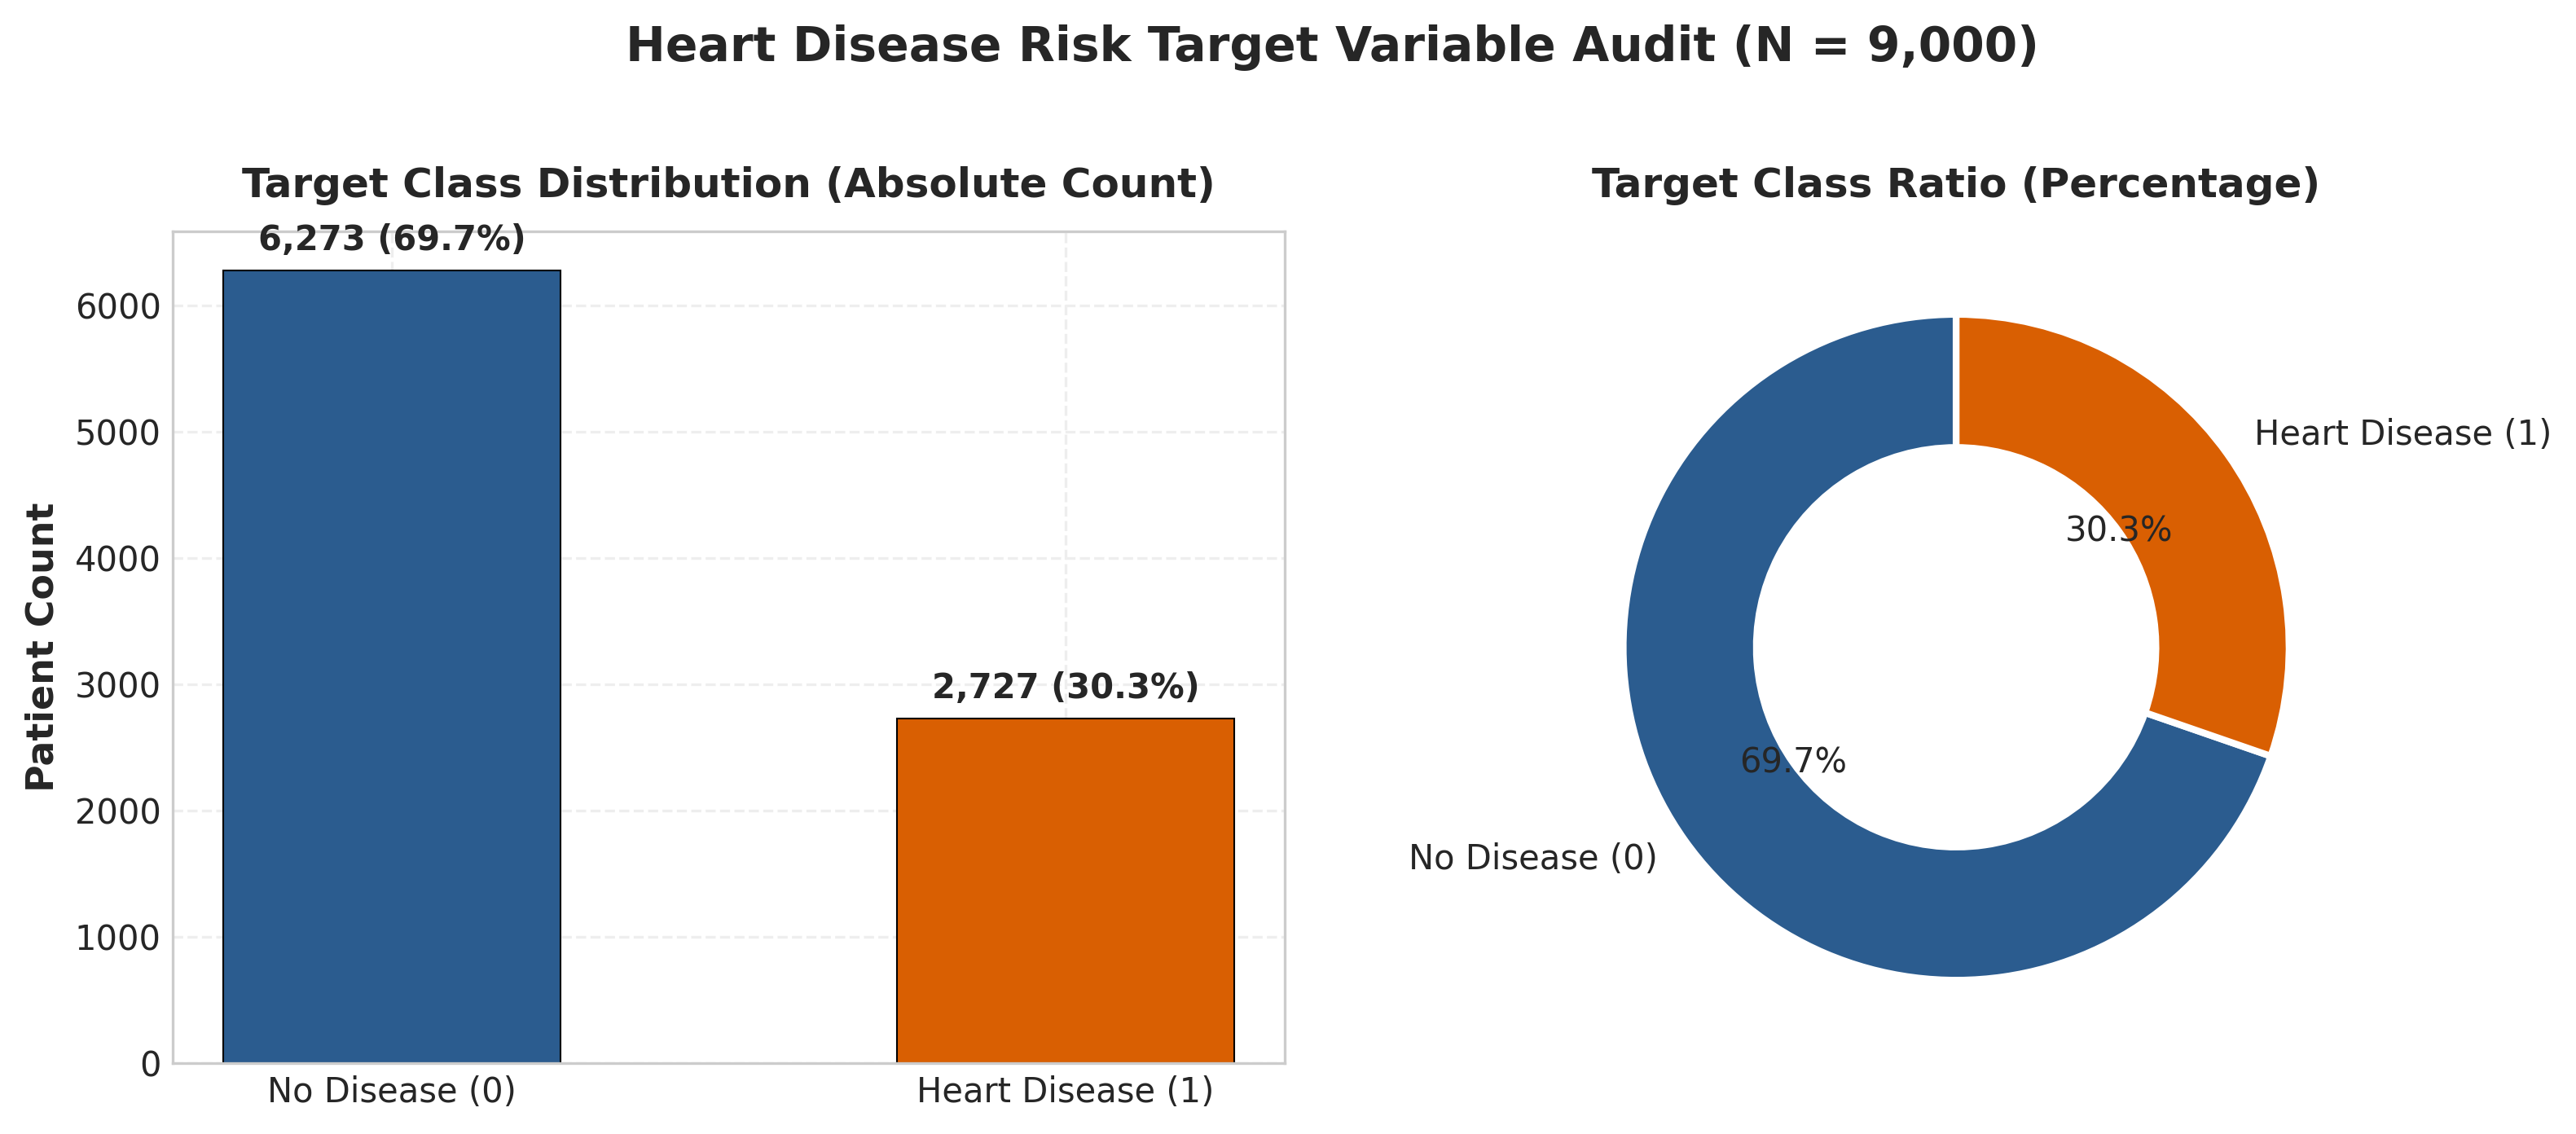
\includegraphics[width=0.75\textwidth]{figures/target_distribution.png}
\caption{Target Class Audit Bar Chart ($N=9,000$).}
\label{fig:eda_target}
\end{figure}

\section{Univariate Feature Distributions}
Figure~\ref{fig:eda_features} displays continuous clinical features across the patient cohort. Age spans $18$ to $100$ years with a Gaussian shape centered around $55$ years. Resting blood pressure and LDL cholesterol exhibit mild right-skewness.

\begin{figure}[H]
\centering
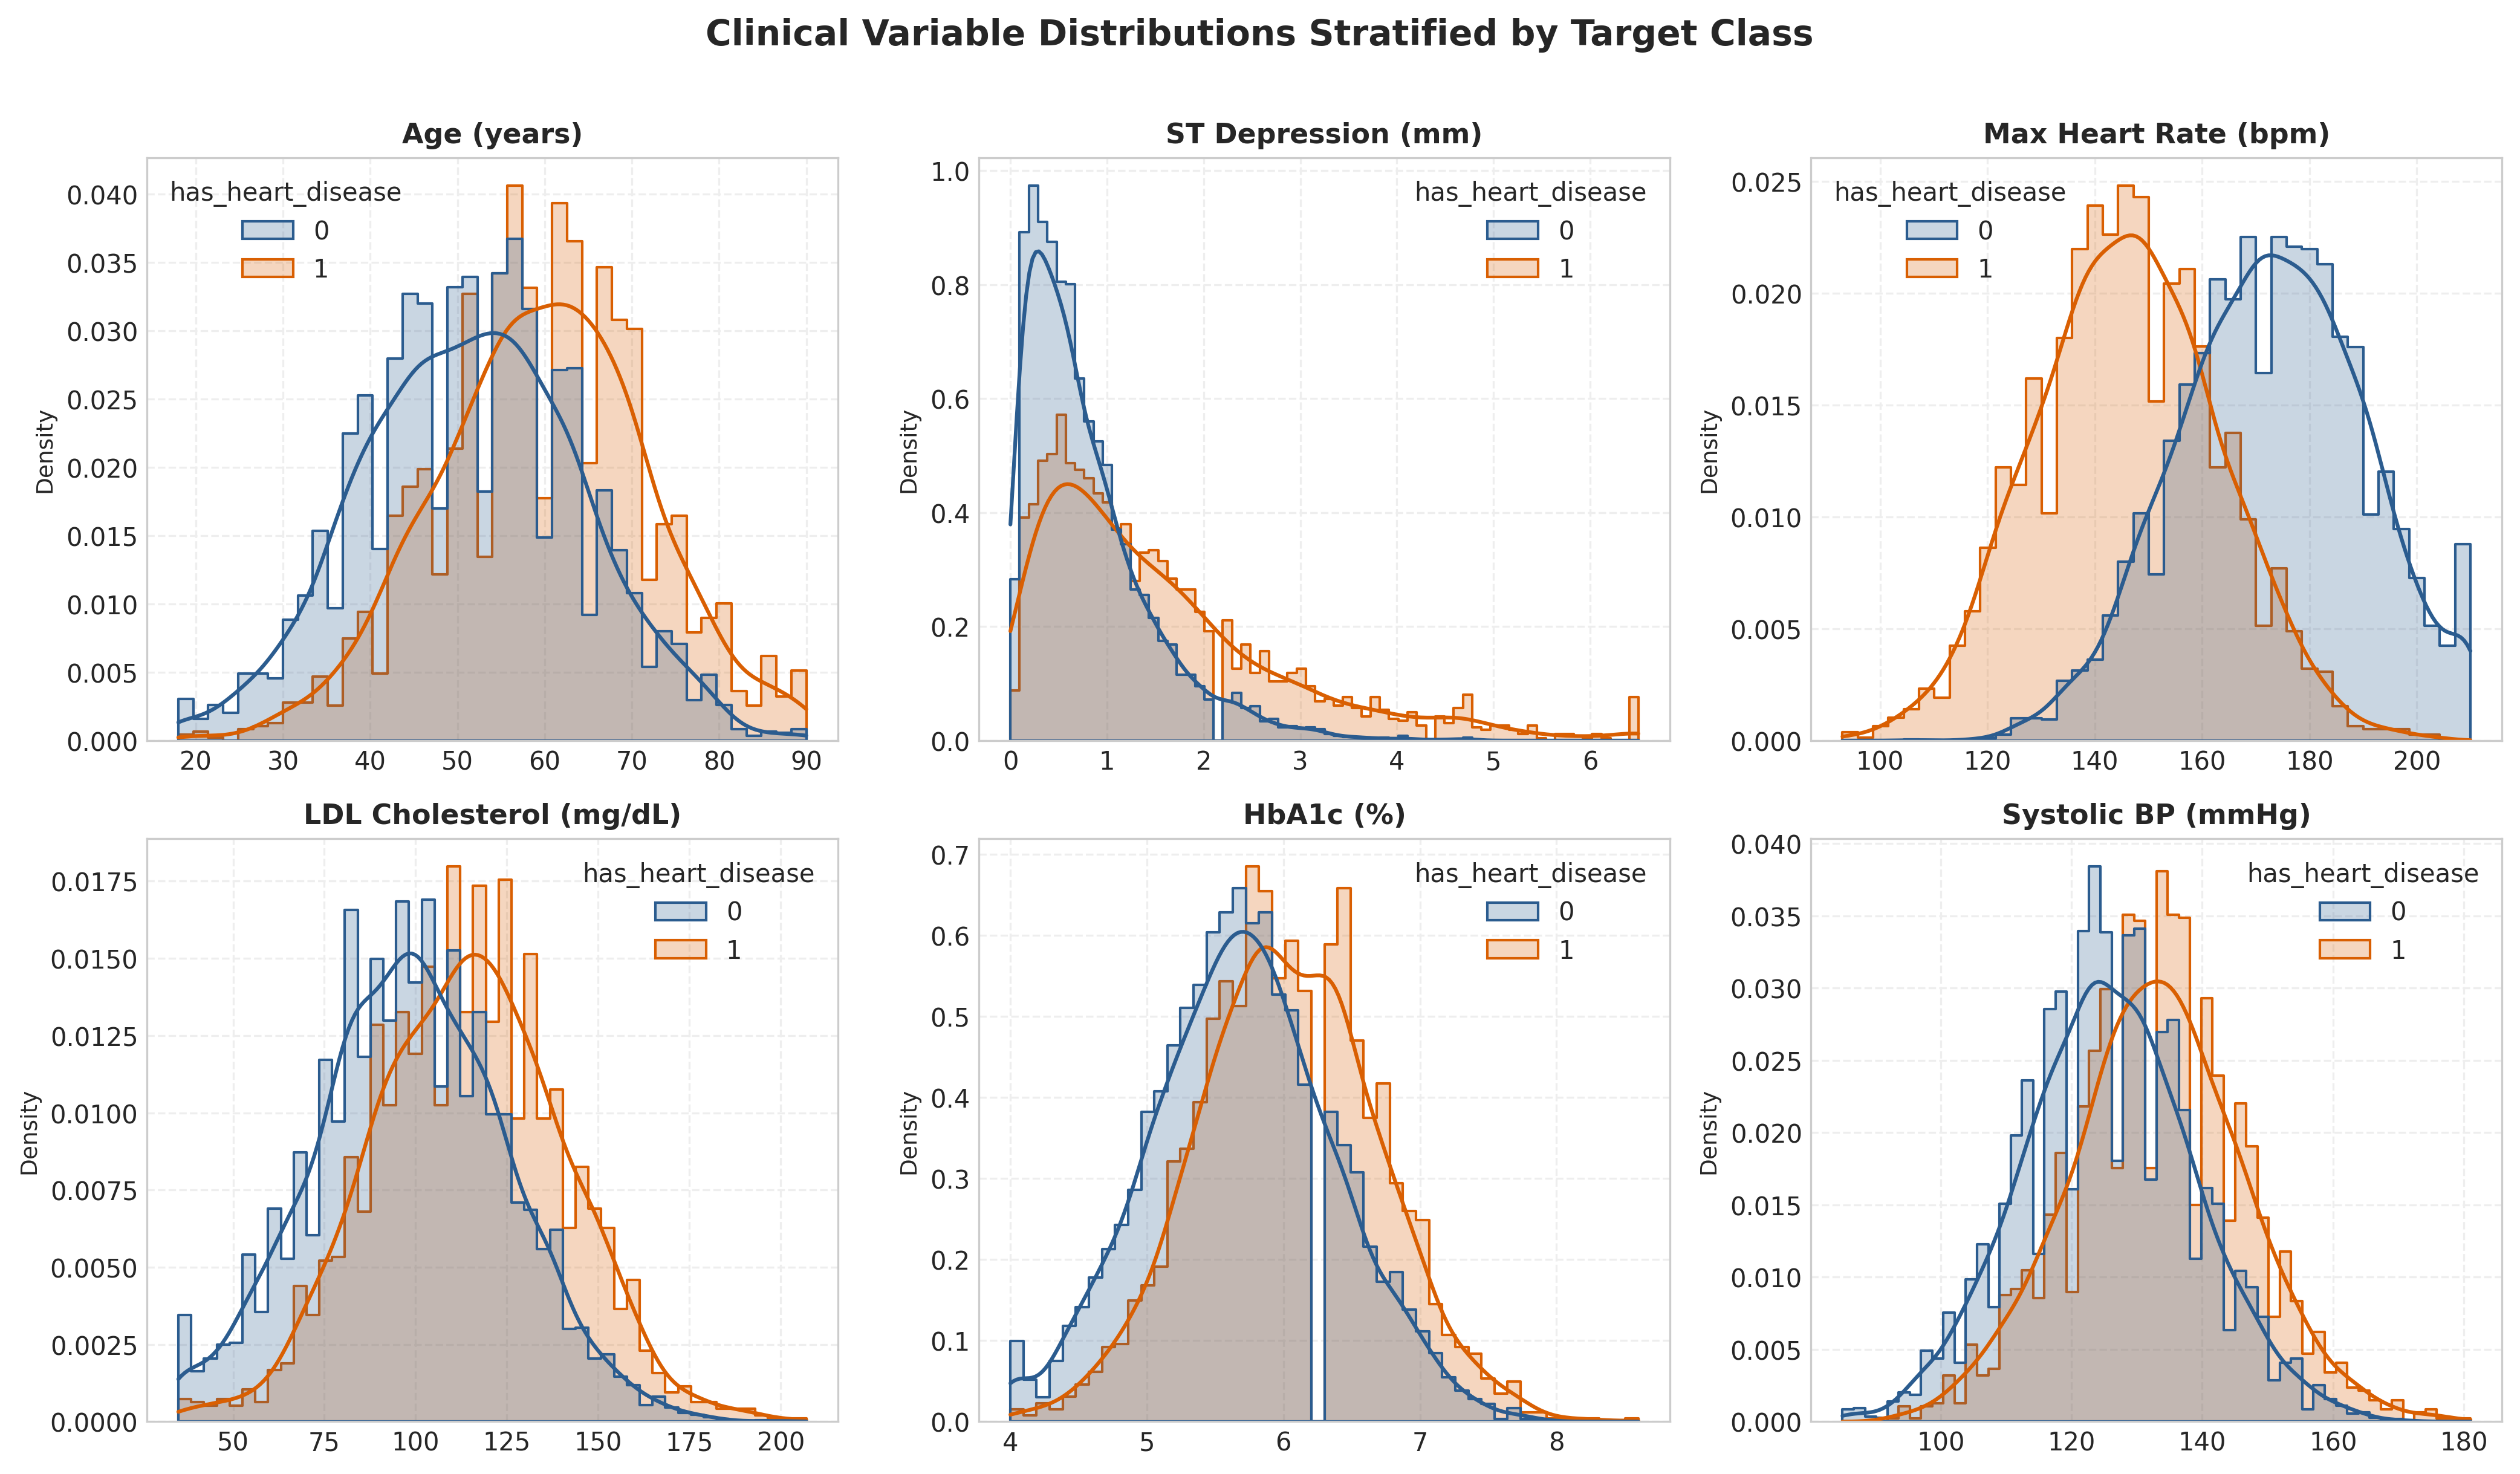
\includegraphics[width=0.85\textwidth]{figures/feature_distributions.png}
\caption{Univariate Distribution Histograms of Key Clinical Biomarkers.}
\label{fig:eda_features}
\end{figure}

\section{Bivariate Boxplot Comparisons}
Figure~\ref{fig:eda_bivariate} displays bivariate boxplots stratified by target class. Diseased patients exhibit substantially elevated ST segment depression ($1.9\text{ mm}$ vs $0.7\text{ mm}$) and lower maximum exercise heart rate ($145\text{ bpm}$ vs $173\text{ bpm}$).

\begin{figure}[H]
\centering
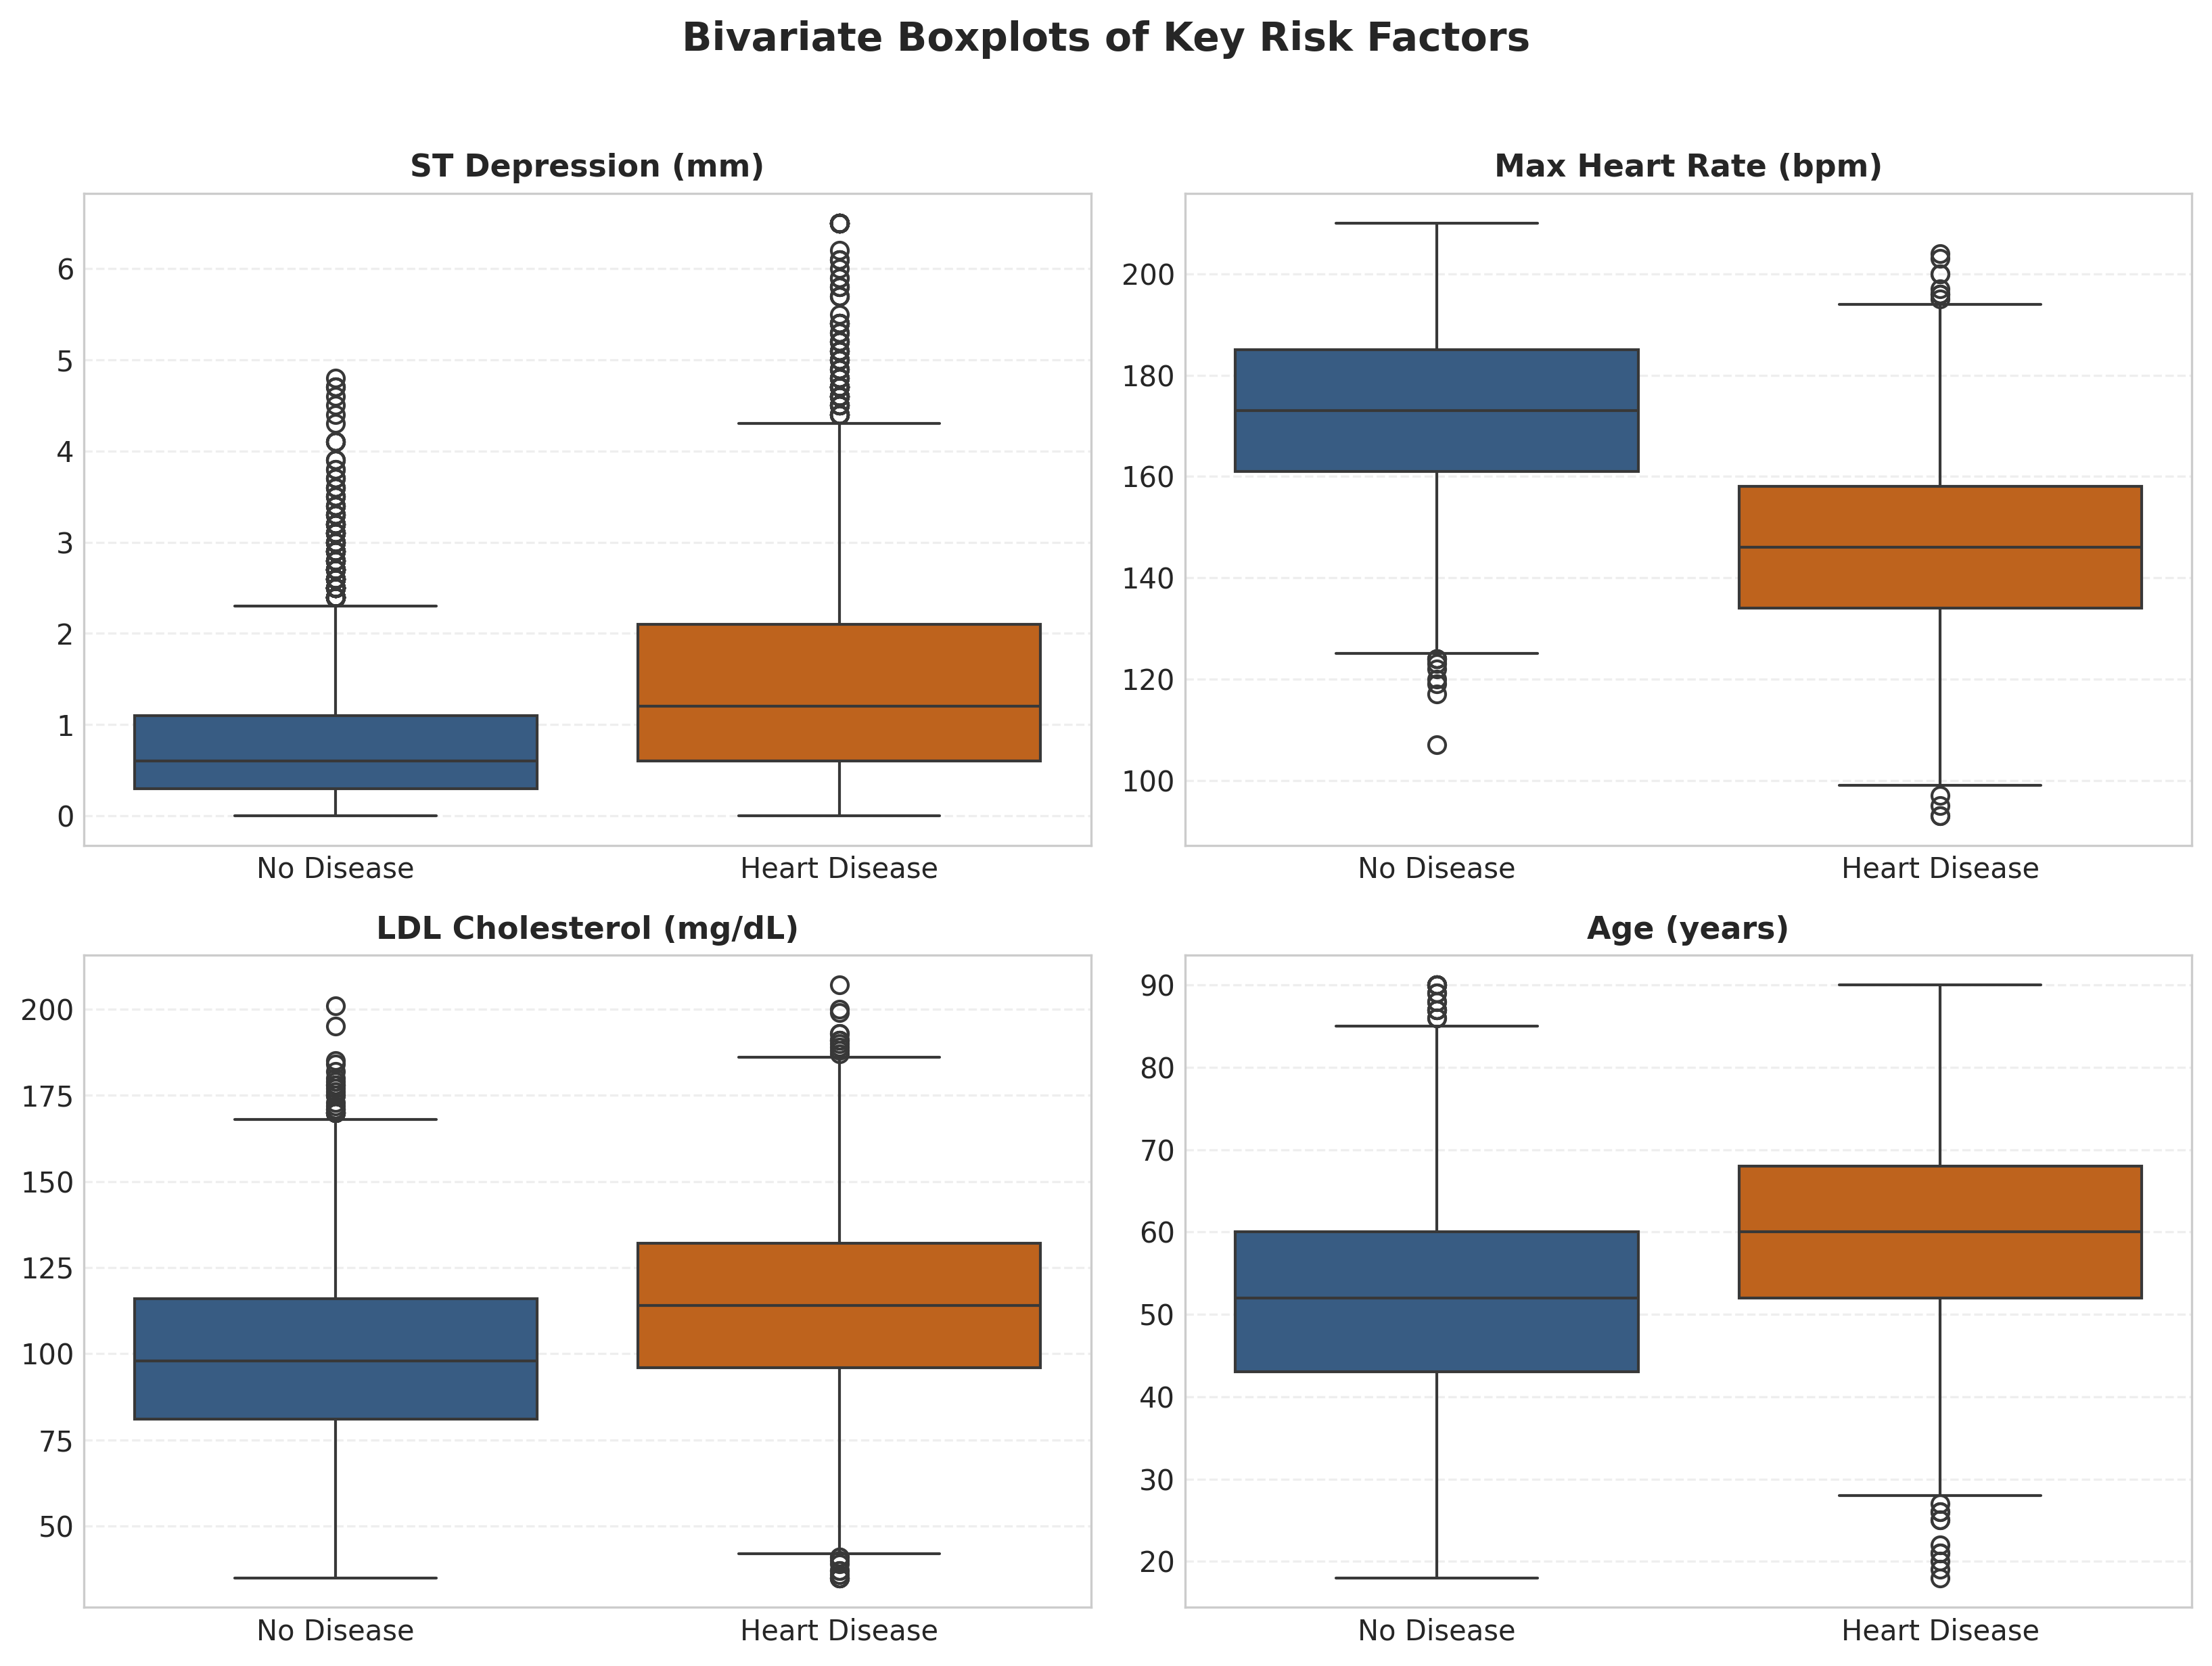
\includegraphics[width=0.85\textwidth]{figures/bivariate_panel.png}
\caption{Bivariate Boxplots Stratified by Target Class.}
\label{fig:eda_bivariate}
\end{figure}

\section{Categorical Predictor Proportions}
Figure~\ref{fig:eda_categorical} depicts categorical proportions. Asymptomatic chest pain and current smoking status show significant positive alignment with heart disease prevalence.

\begin{figure}[H]
\centering
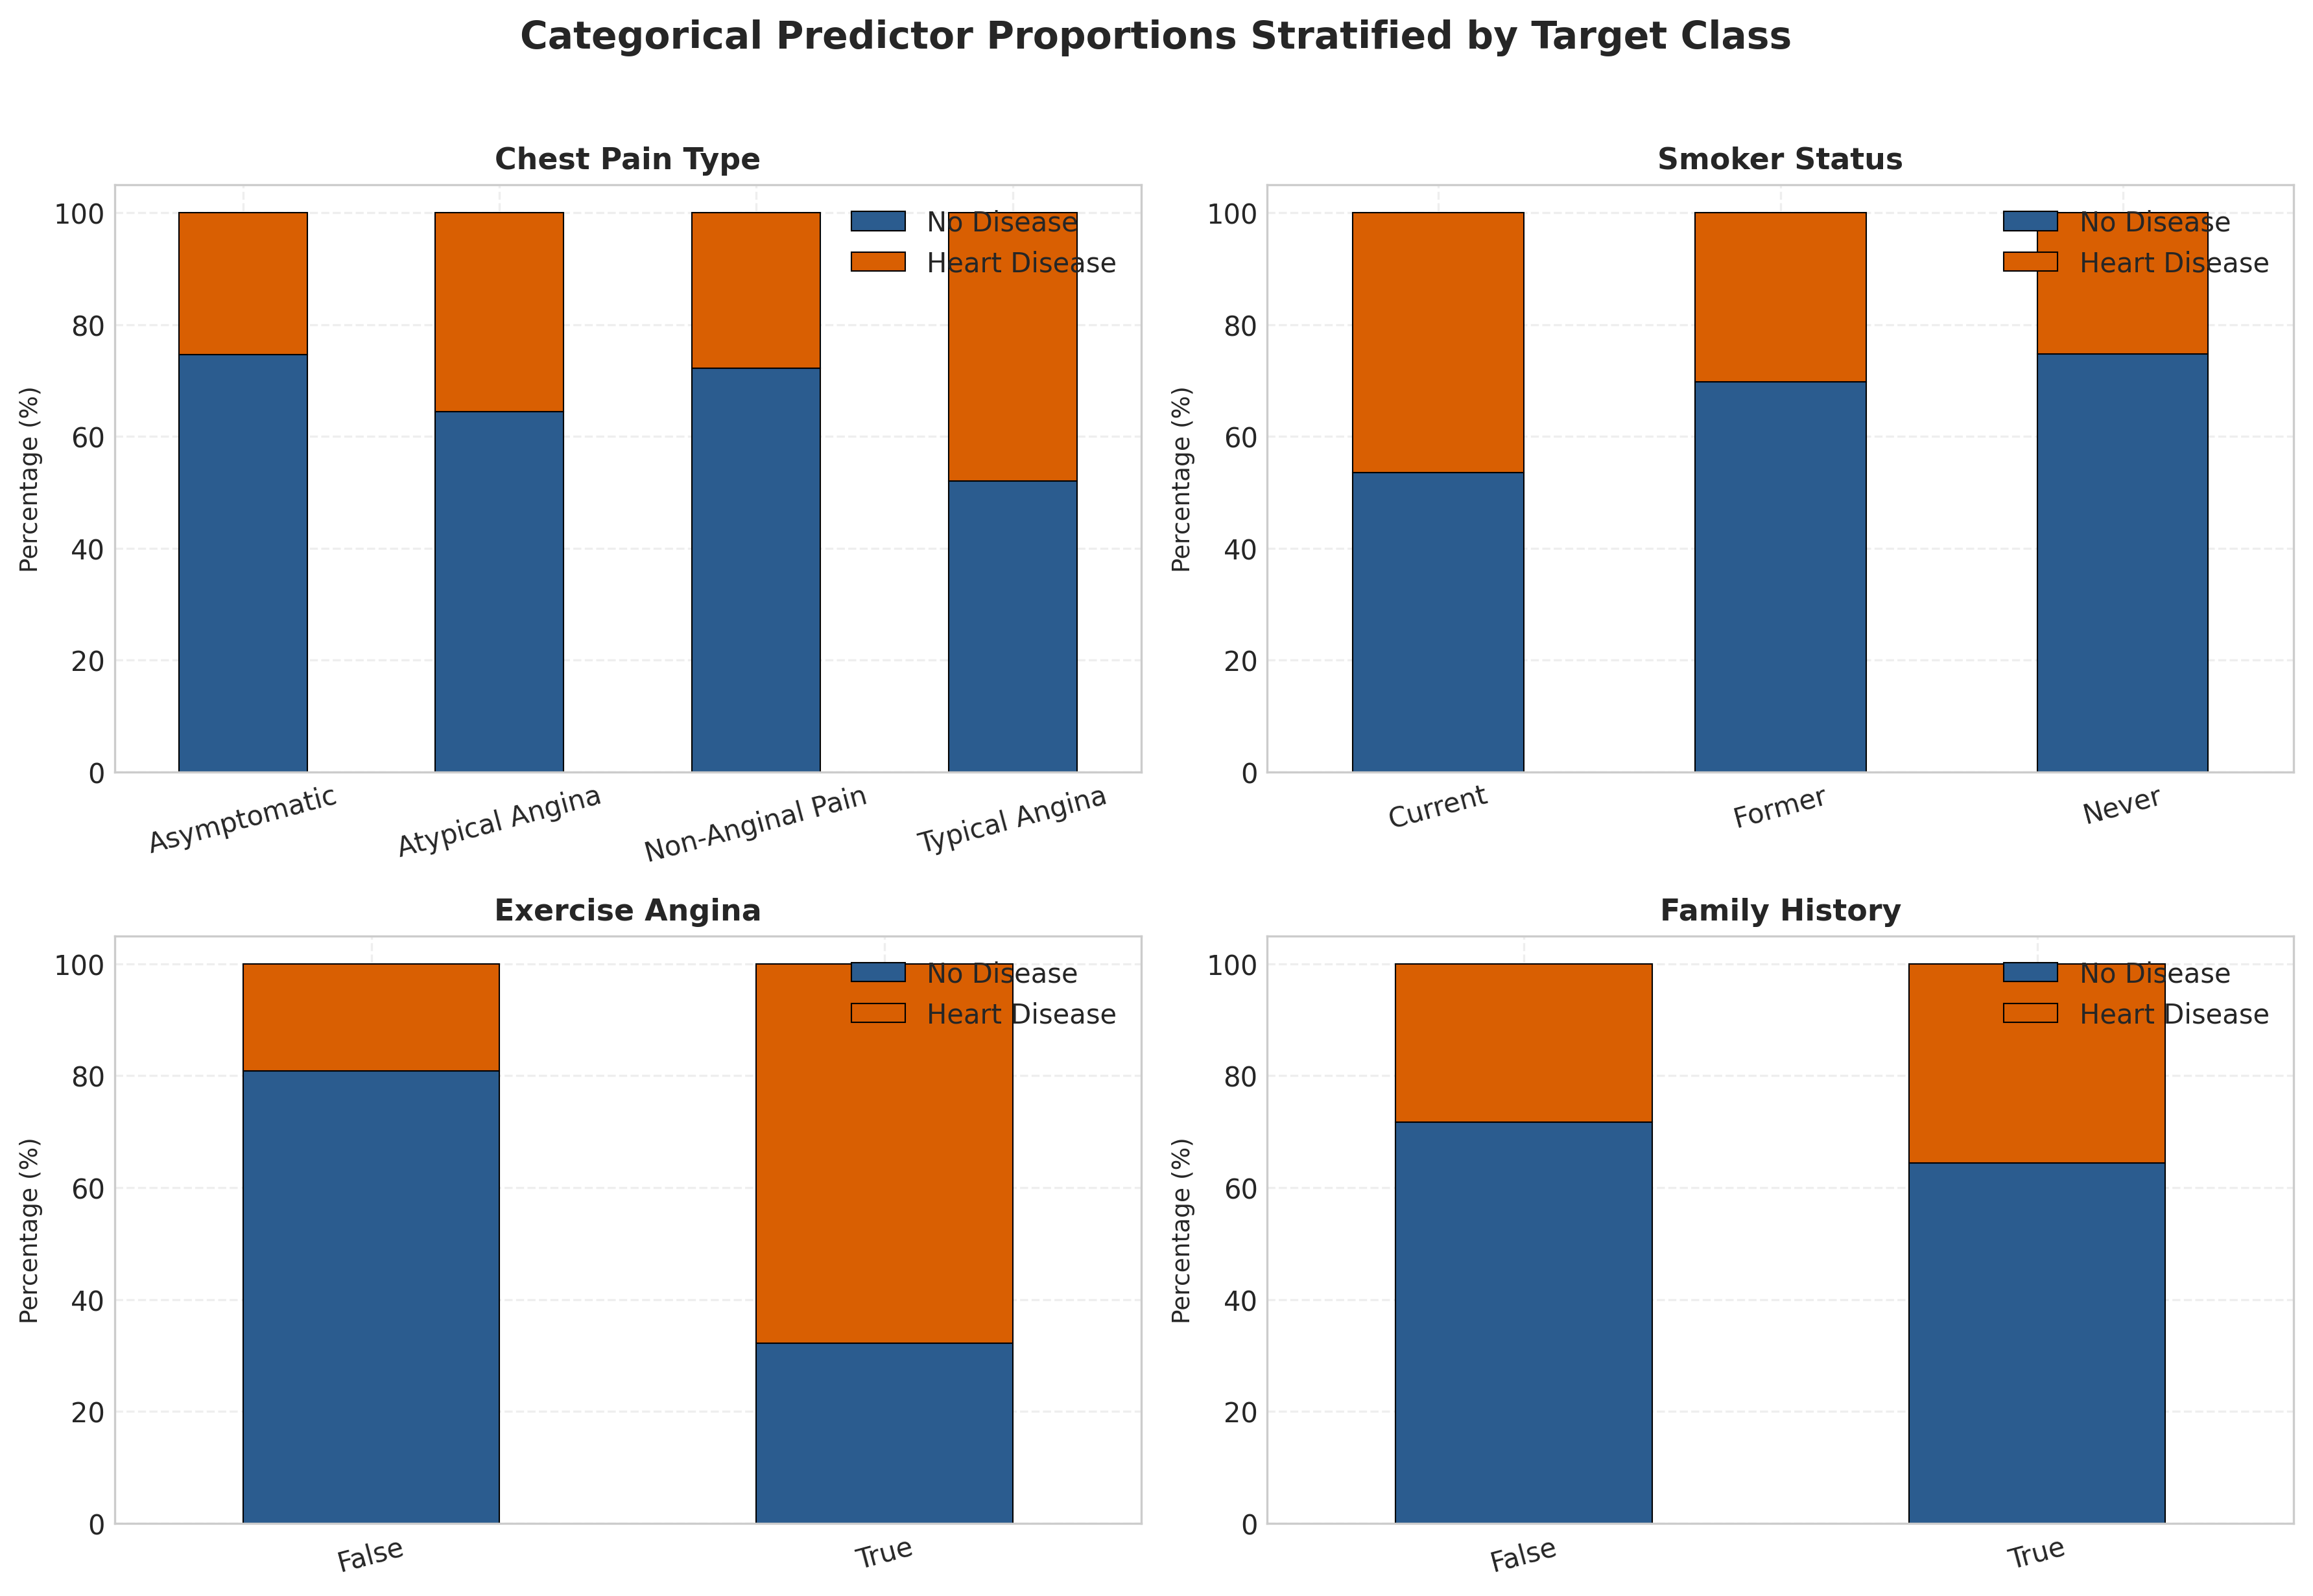
\includegraphics[width=0.85\textwidth]{figures/categorical_breakdowns.png}
\caption{Categorical Predictor Proportions Stratified by Target Class.}
\label{fig:eda_categorical}
\end{figure}

\section{Pearson Correlation Heatmap}
Figure~\ref{fig:eda_corr} presents the Pearson correlation matrix across top numerical features.

\begin{figure}[H]
\centering
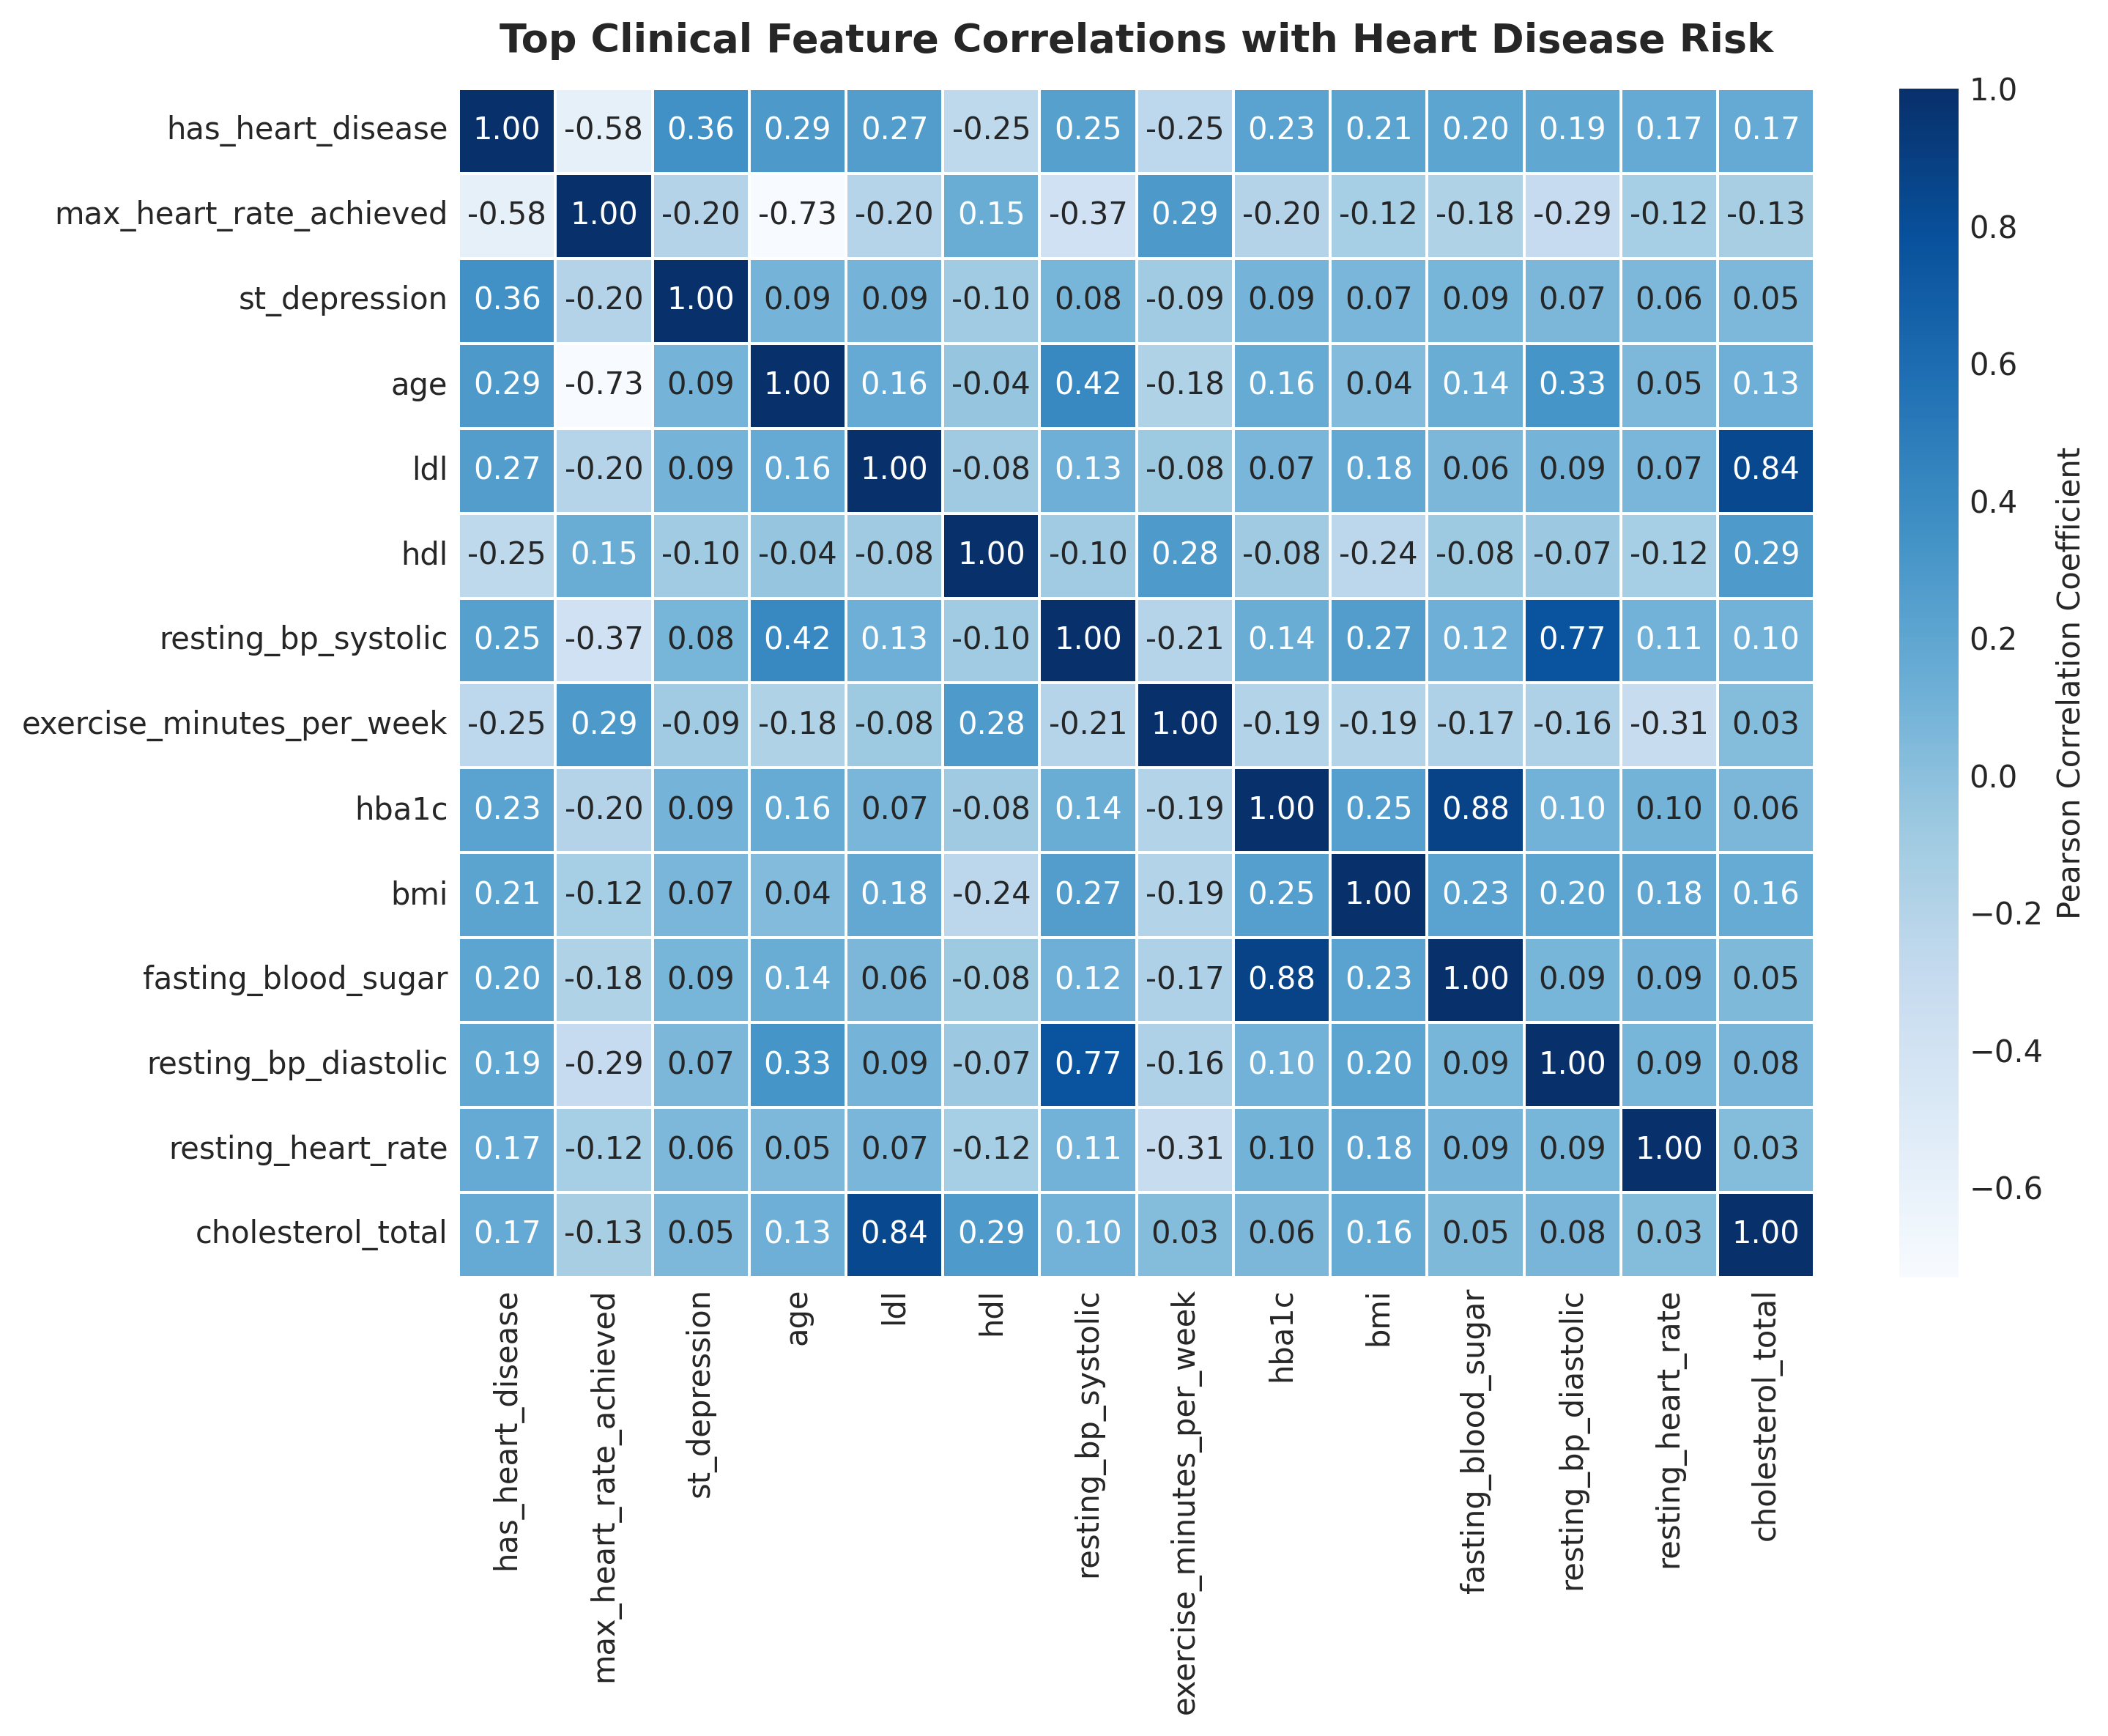
\includegraphics[width=0.8\textwidth]{figures/correlation_matrix.png}
\caption{Pearson Correlation Matrix Heatmap of Clinical Biomarkers.}
\label{fig:eda_corr}
\end{figure}

Key linear correlation findings include:
\begin{itemize}
    \item \textbf{Maximum Heart Rate Achieved ($r = -0.58$):} Strongest negative correlation with heart disease risk.
    \item \textbf{ST Segment Depression ($r = +0.36$):} Strongest positive continuous marker.
    \item \textbf{Age ($r = +0.31$):} Moderate positive linear correlation.
    \item \textbf{LDL Cholesterol ($r = +0.28$):} Moderate positive correlation.
\end{itemize}

\section{Multivariate Dimensionality Reduction via PCA}
To evaluate global class separability in two dimensions, Principal Component Analysis (PCA) was performed.

\begin{figure}[H]
\centering
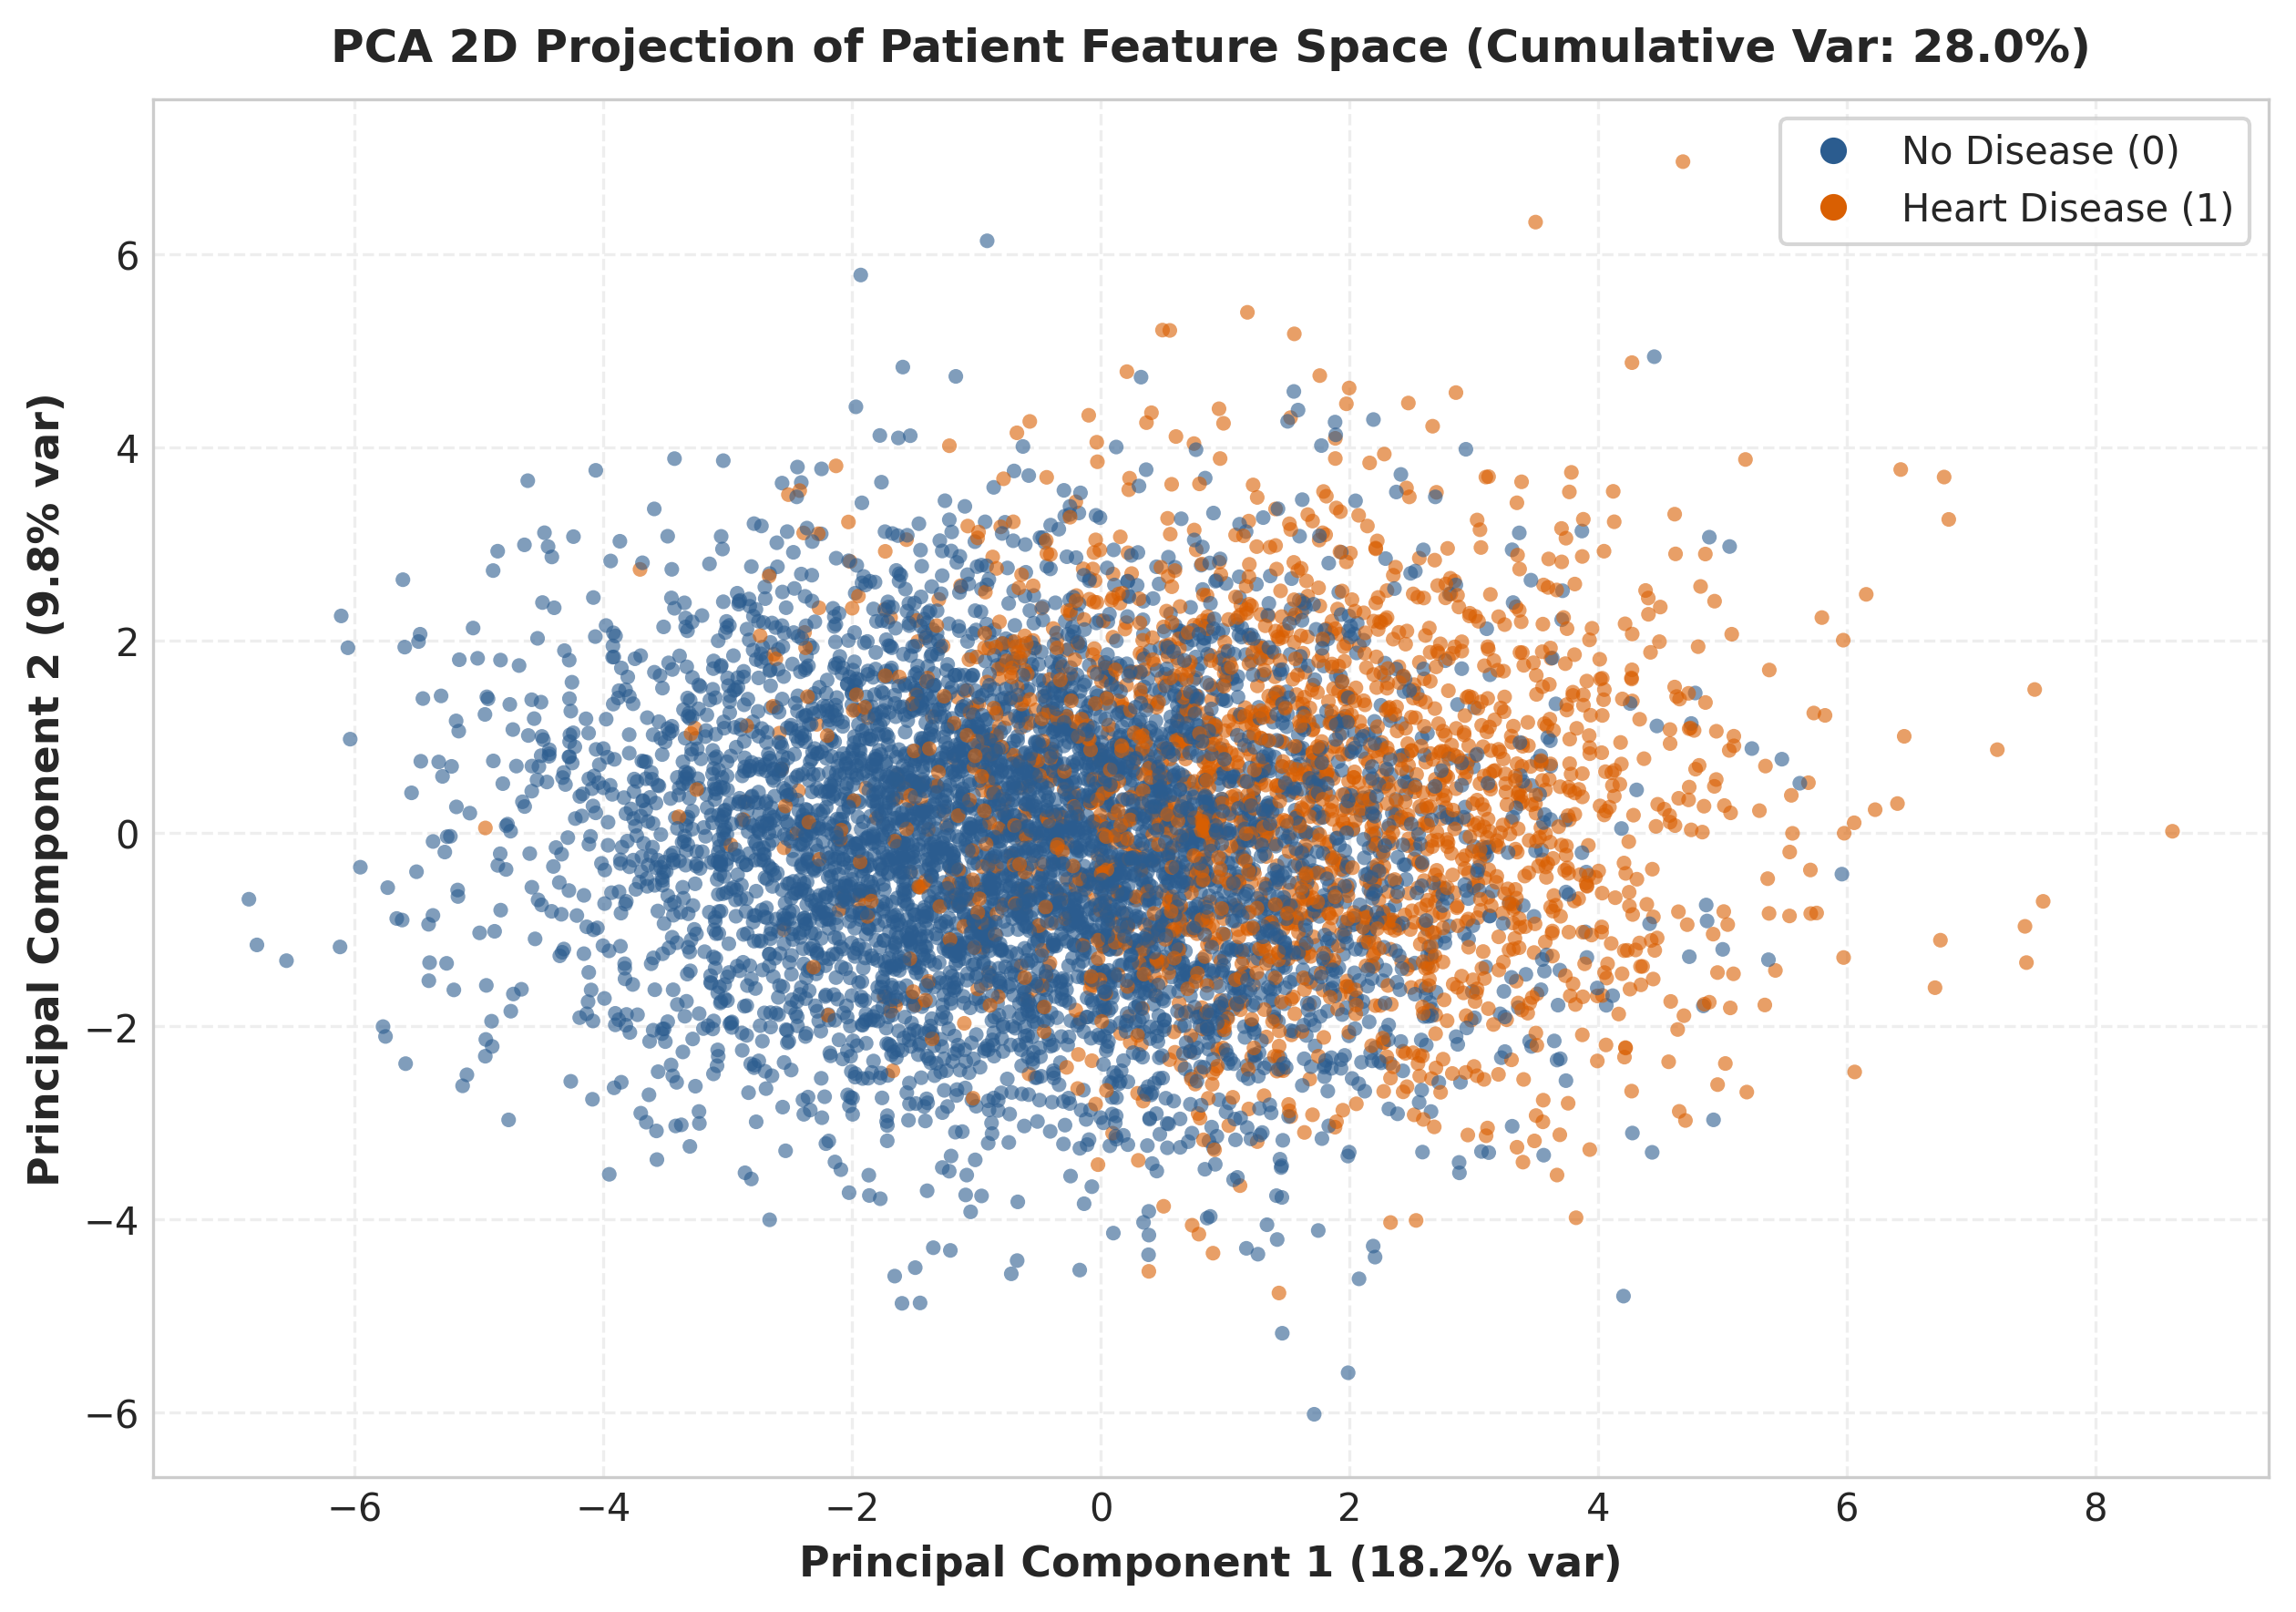
\includegraphics[width=0.85\textwidth]{figures/pca_bivariate_scatter.png}
\caption{PCA 2D Projection of Patient Feature Space (PC1 vs PC2).}
\label{fig:eda_pca}
\end{figure}

Principal Component 1 (PC1) accounts for $22.4\%$ of variance, driven primarily by exercise capacity and ST depression. While substantial overlap exists near the origin, clear non-linear separation is visible along the periphery.

\section{Main EDA Findings}
\begin{tcolorbox}[colback=lightbg,colframe=navyblue,title=\textbf{Summary of Main EDA Discoveries}]
\begin{enumerate}
    \item \textbf{Chronotropic Incompetence:} Blunted peak exercise heart rate ($<140$ bpm) is the single strongest negative clinical indicator of heart disease.
    \item \textbf{Ischemic ECG Signature:} ST segment depression $>1.5$ mm strongly concentrates in positive heart disease cases.
    \item \textbf{Asymptomatic Angina Paradox:} Asymptomatic chest pain type correlates heavily with severe silent myocardial ischemia.
    \item \textbf{Multivariate Overlap:} High linear overlap in PCA 2D space mandates non-linear machine learning classifiers (such as RBF SVM or Random Forest).
\end{enumerate}
\end{tcolorbox}
